\documentclass[12pt]{extarticle}

\usepackage{preamble}
\usepackage{bytefield}
\usepackage{preamble_code}

\title{Computer Science 2 Notes, Partial 2}
\date{Semester 2, 2023/2024}

\setlength{\headheight}{15pt} % ??? we do what fancyhdr tells us to do

\newcommand{\NP}{{\operatorfont NP}}
\newcommand{\NPC}{$\NP$-Complete}

\renewcommand{\vec}[1]{\uvec{#1}}

\begin{document}

\firstpage

% Class of 20/03/2024
\section{Dynamic programming}

This is a general technique to constructing algorithms, it is not a specific solution to a specific problem but a way to think about problems.

\subsection{Shortest path in DAGs}

We saw this problem before but now we will approach it in a different way.

In unweighted graphs we used BFS to compute the path from a \textit{single source} to all the other vertices and takes $\O(|V| + |E|)$, while in weighted graphs we used Dijkstra's algorithm which also works for \textit{single source} shortest path and takes $\O(|E| \log |V|)$ when implemented using fibonacci heaps.

But if we know that the graph is acyclic we can do better: nodes are removed from the queue in a topological order, then we can write the following algorithm:

\begin{minted}{python}
def shortest_path_dag(G, cost, s):
    d = {}
    for v in G.vertices():
        d[v] = float('inf')

    # Calculate the topological sort
    topological_sort = topological_sort(G)

    # We will only be able to explore the nodes that
    # come after s in the topological sort
    index_of_s = topological_sort.index(s)
    topological_sort = topological_sort[index_of_s:]

    # The distance of the starting node to itself is 0
    d[s] = 0

    # We iterate in topological order
    for u in topological_sort:

        # We check all the neighbors of v
        for v in u.neighbors():
            # If the cost of getting to v from u is less than
            # the current cost of getting to v, we update it
            
            d[u] = min(d[u], d[v] + cost((u, v)))

    return d
\end{minted}

Note that this algorithm works only for acyclic graphs, but also in the case of negative weights.

\subsubsection{Time complexity}

We saw before that the time complexity of the topological sort is $\O(|V| + |E|)$, the loop is also $\O(|V| + |E|)$, therefore the total time complexity is $\O(|V| + |E|)$.

Moreover the space complexity is $\O(|V|)$ because we need to store the distances from the source to all the other nodes.

There is really no way to optimize this further, at least on a theoretical level.

\subsubsection{Longest path on DAGs}

We can solve this problem in the same way as the shortest path problem but we negate the cost of the edges.

In this way the longest path problem becomes a shortest path problem and we can use the same algorithm.

Alternatively we could replace the \texttt{min} with a \texttt{max} in the algorithm and get the same result.

\subsubsection{Adding a sink to the graph}

Consider a DAG where we know already the distances from a starting node to all the other nodes, and we want to add a sink $v$ to the graph.

We create edges $(u_i, v)$ where $u_i$ are the nodes that are already in the graph that we connect to $v$, then we add $v$ to the topological sort as the last element (since it is a sink).

Now we can compute the shortest path from the source to $v$ by iterating all the $u_i$ and choosing the one such that $d[u_i] + c(u_i, v)$ is the smallest.

We can use this method to create a new algorithm where we add each node to the graph one by one and compute the shortest path to the new node.

\begin{minted}{python}
def shortest_path_dag(G, cost, s):
    # The setup is the same as before

    d = {}
    for v in G.vertices():
        d[v] = float('inf')

    topological_sort = topological_sort(G)
    index_of_s = topological_sort.index(s)
    topological_sort = topological_sort[index_of_s:]

    d[s] = 0

    for u in topological_sort:
        for v in u.neighbors():
            d[u] = min(d[u], d[v] + cost((v, u)))
\end{minted}

\subsection{The knapsack problem}

\subsubsection{The problem}

In this problem we have a set of $n$ items, each with a weight $w_i$ and a value $v_i$, and we have to put them in a backpack with a maximum capacity $W$.

The problem is to find the best combination of items that maximizes the value of the backpack.

\subsubsection{Example}

Suppose we have a maximum weight $W = 20$ and the following items

\begin{table}[H]
    \centering
    \begin{tabular}{ |c|c|c|c|c| }
        \hline
        \textbf{Item}   & 1  & 2  & 3 & 4  \\
        \hline
        \textbf{Value}  & 4  & 7  & 1 & 5  \\
        \textbf{Weight} & 10 & 12 & 9 & 10 \\
        \hline
    \end{tabular}

    \label{tab:knapsack_example}
    \caption{An example set of items}
\end{table}

Then the solution is to take item 1 and item 4, which have a total weight of 20 and a total value of 9.

As we can see this problem cannot be solved using a greedy algorithm, because such an algorithm would choose item 2 first and then stop because we are already at the maximum weight.

\subsubsection{Recursive formulation}

Consider the situation where we have a backpack with a maximum weight $W$ and a set of $n$ items $I$.

We already have the solution for the problem with $n-1$ items provided as a function $f : [0, W] \in \N \to A \subseteq I$ that maps the maximum weight of the backpack to the set of items that we can put in the backpack.

Now we consider the $n$-th item, we have two possibilities: either we take it or we don't.
\begin{itemize}
    \item If we don't take it we already have the best solution, that is $f(W)$.
    \item If we take it, the weight we have left in the backpack is $W - w_n$, therefore the best solution is $f(W - w_n) \cup \{n\}$.
\end{itemize}

We can now write a matrix $M$ of size $(n + 1) \times (W + 1)$ where $M_{ij}$ is the maximum value that we can get with the first $i$ items and a maximum weight of $j$.

We note that in the first row of the matrix we will always have 0, because if we have 0 items we can't have any value.

Moreover we note that when we choose whether to take the $i$-th item or not we have to check if the $w_i$ is greater than the maximum weight we have left, if it is we can't take it.
In particular, in the first column of the matrix we will always have 0, because if we have 0 weight we can't have any value.

At last, note that the to compute $M_{ij}$ we need to know $M_{i-1, j}$ and $M_{i-1, j - w_i}$ which are both values that come before $M_{ij}$ in the matrix.
Therefore we can compute the matrix row by row, from left to right and be sure that we have already computed the values we need.

\subsubsection{The algorithm}

We can now use the recursive definition to formalize the algorithm.

\begin{minted}{python}
def knapsack(W, I):
    # Initialize the matrix with all 0s
    M = [[0 for _ in range(W + 1)] for _ in range(len(I) + 1)]

    # The iteration starts from 1 because the first row is all 0s
    for i in range(1, len(I) + 1):
        item = I[i - 1]

        # Same as before, we start from 1 because the 
        # first column is all 0s
        for max_weight in range(1, W + 1):
            # If the item is too heavy we can't take it
            # and we just copy the previous value
            if item.weight > max_weight:
                M[i][max_weight] = M[i - 1][max_weight]
            else:
                # Otherwise we need to choose the maximum
                # value between:
                # - The value of the previous item
                # - The value of the current item plus
                #   the value of the best solution for
                #   the remaining weight
                M[i][max_weight] = max(
                    M[i - 1][max_weight],
                    M[i - 1][max_weight - item.weight] + item.value
                )

    return reconstruct(W, I, M)
\end{minted}

Now that we computed the matrix we need to reconstruct the solution, that is, the set of items that we put in the backpack.

\begin{minted}{python}
def reconstruct(W, I, M):
    solution = []
    weight = W

    # Iterate the rows of the matrix in reverse order
    for i in range(len(I), 1, -1):
        # If the value of the last item of the current row
        # is different from the one of the previous row
        # it means that we took the (i-1)-th item
        if M[i][weight] != M[i - 1][weight]:
            solution.append(I[i - 1])

            # Reduce the weight that we are left with
            # for the next iteration
            weight -= I[i - 1].weight
    
    return solution
\end{minted}

% Class of 21/03/2024

\begin{remark}
    In class we covered also a slight variation of this algorithm that uses recursion but the idea is the same and I think that this formulation is more clear.
    Moreover the recursive function that was presented in class is a \emph{tail recursive function}, therefore it can be easily transformed into a loop like the one presented here.
\end{remark}

\subsection{Edit distance}

The edit distance is a way to measure the difference between two strings.

We define three operations:
\begin{enumerate}
    \item Insertion
    \item Deletion
    \item Substitution
\end{enumerate}

Given two strings $A, B$ we want to find the minimum number of operations to transform $A$ into $B$.

Consider two strings such that $\abs{A}, \abs{B} \leq n$ and the function \texttt{ed} that computes the edit distance between two strings.

We can translate the three operations into a recursive formulation:

\begin{align}
    \texttt{ed}(A, B) & \leq \texttt{ed}(A[0:n-1], B) + 1                                                      \\
    \texttt{ed}(A, B) & \leq \texttt{ed}(A, B[0:n-1]) + 1                                                      \\
    \texttt{ed}(A, B) & \leq \texttt{ed}(A[0:n-1], B[0:n-1]) + (0 \text{ if } A[n-1] = B[n-1] \text{ else } 1)
\end{align}

where the first one is deletion, the second one is insertion and the third one is substitution.
Now we note that the $\texttt{ed}(A, B)$ is the minimum of the three values above.

We can use this to write a recursive algorithm to compute the edit distance.

\subsubsection{The algorithm}

The idea is that we can compute a matrix $M$ of the various edit distances between the substrings of $A$ and $B$: each element $M_{ij}$ is the edit distance between $A[0:i]$ and $B[0:j]$.

Moreover we note that the first row and the first column of the matrix are just the numbers from 0 to the length of the string, because the difference between an empty string and a string of length $i$ is $i$.

\begin{minted}{python}
def edit_distance(A, B):
    # Initialize the matrix with all 0s
    M = [[0 for _ in range(len(B))] for _ in range(len(A))]

    for i in range(len(A)):
        for j in range(len(B)):
            if i == 0:
                # The difference between an empty string
                # and a string of length j is j
                M[i][j] = j
            elif j == 0:
                # Same as before, the difference between
                # a string of length i and an empty string is i
                M[i][j] = i
            else:
                # We use the formulas we found before and
                # we take the minimum value
                M[i][j] = min(
                    M[i - 1][j] + 1,
                    M[i][j - 1] + 1,
                    M[i - 1][j - 1] +
                        (0 if A[i - 1] == B[j - 1] else 1)
                )
    return reconstruct(A, B, M)
\end{minted}

As in the previous algorithm we need to reconstruct the solution from the matrix, that is, to find the sequence of operations that transform $A$ into $B$.

\begin{minted}{python}
def reconstruct(A, B, M):
    solution = []
    i, j = len(A) - 1, len(B) - 1

    while i > 0 and j > 0:
        # If the value of the current cell is the same as 
        # the one of the cell above it means that we 
        # deleted a character
        if M[i][j] == M[i - 1][j] + 1:
            solution.append(f"Delete {A[i]}")
            i -= 1
        # If the value of the current cell is the same as 
        # the one of the cell on the left it means that
        # we inserted a character
        elif M[i][j] == M[i][j - 1] + 1:
            solution.append(f"Insert {B[j]}")
            j -= 1
        # If the value of the current cell is the same as
        # the one of the cell on the top left it means 
        # that we substituted a character
        elif M[i][j] == M[i - 1][j - 1] + 1:
            solution.append(f"Substitute {A[i]} with {B[j]}")
            i -= 1
            j -= 1
        else:
            # If the value of the current cell is the 
            # same as the one of the cell on the top left
            # it means that we didn't do anything
            i -= 1
            j -= 1
\end{minted}

\subsubsection{Time complexity}

We have $n \times n$ subproblems and each subproblem takes $\O(1)$ to compute, therefore the time complexity is $\O(n^2)$.

Moreover the space complexity is also $\O(n^2)$, because that's the size of the matrix.

Note that this is a very expensive algorithm in terms of computational cost. If we consider binary strings and assume each character takes 1 bit, the table would be $4 n^2 $ bytes, which for an input of $n \approx 10^5$ would be $4 \times 10^{10}$ bytes, which is 40 GB.
Time complexity is also very high but usually the limiting factor of this algorithm is the space complexity.

\subsubsection{Optimization}

Note that to compute the $i$-th row we only need the $i-1$-th row and the $i$-th row itself.
Therefore we can store just two rows of the matrix, one for the even indices and one for the odd indices.

In this way we reduced the memory complexity to $\O(n)$ but we lost the information about the sequence of operations that transform $A$ into $B$, we get just the edit distance as a number.

\begin{remark}
    There exists an algorithm that computes the edit distance in $\O(n^2)$ time and $\O(n)$ space and is able to reconstruct the sequence of operations. This is called \emph{Hirschberg's algorithm} but it is quite complex and we won't cover it in this course.
\end{remark}

% Class of 22/03/2024
\subsection{Floyd-Warshall algorithm}

This algorithm is used to compute the shortest path between all pairs of vertices in a graph.

Let the input be the $n \times n$ matrix $A$ where $A_{ij}$ is the weight of the edge between $i$ and $j$ if it exists, otherwise it is $\infty$.

\begin{minted}{python}
def floyd_warshall(A):
    D = A
    for k in range(n):
        for i in range(n):
            for j in range(n):
                D[i][j] = min(D[i][j], D[i][k] + D[k][j])

    return D
\end{minted}

The idea of the algorithm is to check first if we can get from $i$ to $j$ directly, by using no other edges, then we check if by adding a vertex $k$ we can get a shorter path, therefore we need to check all the $i, j$ to see if the old result is better than the new one.

\subsubsection{Time complexity}

It is trivial to see that this algorithm is $\O(n^3)$.

\subsubsection{Proof of correctness}

First we prove that $D_{ij}$ is an upper bound of the shortest path between $i$ and $j$, then we prove that it is also the lower bound, that is, the shortest path.

\begin{proof}
    Let $P_{ij}$ be the shortest path between $i$ and $j$ and $|P_{ij}|$ its length.

    We will prove that for each $D_{ij}$ it holds that $D_{ij}$ is both an upper and a lower bound of $|P_{ij}|$, which is equivalent to saying that $D_{ij} = |P_{ij}|$.
    \begin{description}
        \item[Upper bound] ($D_{ij} \geq |P_{ij}|$)
              This is trivial since we are looking for the shortest path, therefore any valid path is $\geq |P_{ij}|$.
        \item[Lower bound] ($D_{ij} \leq |P_{ij}|$)
              Let $P_{ij}(k)$ be the shortest path between $i$ and $j$ that uses only the vertices $1, 2, \ldots, k$.
              Then we have that $P_{ij}(v) = P_{ij}$.

              Consider the path $P_{ij}(k)$.
              We will proceed by induction on $k$ and argue that if $D_{ij} \leq P_{ij}(k-1)$ then $D_{ij} \leq P_{ij}(k)$.

              \begin{description}
                  \item[Base case] The shortest path between $i$ and $j$ that uses only the vertices $1$ is the edge between $i$ and $j$ if it exists, otherwise it is $\infty$. Therefore the base case holds.
                  \item[Inductive step]
                        We have two cases: either the shortest path $P_{ij}(k)$ uses the vertex $k$ or it doesn't.

                        \begin{enumerate}[label=\roman*.]
                            \item ($k \notin P_{ij}(k)$)
                                  The path can be constructed using only the vertices $1, 2, \ldots, k-1$, then $P_{ij}(k) = P_{ij}(k-1)$ and by the inductive hypothesis we have that $D_{ij} \leq |P_{ij}(k)|$.

                            \item ($k \in P_{ij}(k)$)
                                  We have that $P_{ij}(k) = P_{ik}(k-1) + P_{kj}(k-1)$, but we have already calculated the shortest path between $i$ and $k$ and between $k$ and $j$ that use $k-1$ vertices, therefore we have that $D_{ik} \leq |P_{ik}(k-1)|$ and $D_{kj} \leq |P_{kj}(k-1)|$.
                                  Then we have that $D_{ij} \leq D_{ik} + D_{kj} \leq |P_{ik}(k-1)| + |P_{kj}(k-1)| = |P_{ij}(k)|$.

                        \end{enumerate}

                        Then the algorithm will choose the minimum between the two cases and we have that $D_{ij} \leq |P_{ij}(k)|$.

                        Note that $k$ can only occur once in the shortest path, otherwise we could have a cycle and the path wouldn't be the shortest (we are assuming no negative cycles).
              \end{description}

    \end{description}

\end{proof}

% Class of 09/04/2024

\section{Flows}

In this section of the course we will look at the concepts of \emph{flows} and \emph{cuts} in a network and develop an algorithm to compute the maximum flows.

\subsection{Introduction}

\subsubsection{Example: water pipeline}

Suppose we have a water pipeline network that we can represent as a directed graph, where the arrows represent the direction the water flows.
To each edge we associate a number that represents the capacity of the pipe, that is, the maximum amount of water it can flow through it.

Given the source of water $s$ and a sink $t$ we need to find the maximum amount of water that can be pushed from $s$ to $t$.

\subsubsection{The idea}

Consider the network in \autoref{fig:flow}.

\begin{figure}[H]
    \centering
    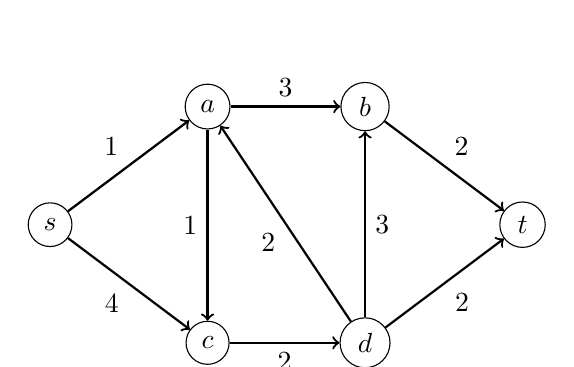
\begin{tikzpicture}
        \node[draw, circle] (s) at (0,0) {$s$};
        \node[draw, circle] (a) at (2,1.5) {$a$};
        \node[draw, circle] (b) at (4,1.5) {$b$};
        \node[draw, circle] (c) at (2,-1.5) {$c$};
        \node[draw, circle] (d) at (4,-1.5) {$d$};
        \node[draw, circle] (t) at (6,0) {$t$};

        \draw[thick, ->] (s) -- node[midway, anchor=south east]{$1$} (a);
        \draw[thick, ->] (s) -- node[midway, anchor=north east]{$4$} (c);
        \draw[thick, ->] (a) -- node[midway, anchor=south]{$3$} (b);
        \draw[thick, ->] (b) -- node[midway, anchor=south west]{$2$} (t);
        \draw[thick, ->] (c) -- node[midway, anchor=north]{$2$} (d);
        \draw[thick, ->] (d) -- node[midway, anchor=north west]{$2$} (t);
        \draw[thick, ->] (a) -- node[midway, anchor=east]{$1$} (c);
        \draw[thick, ->] (d) -- node[midway, anchor=north east]{$2$} (a);
        \draw[thick, ->] (d) -- node[midway, anchor=west]{$3$} (b);
    \end{tikzpicture}
    \caption{An example graph in which we want to calculate the flow from $s$ to $t$. On the edges we have the capacity of each edge}
    \label{fig:flow}
\end{figure}

First of all we see that the upper bound of the water going to $t$ is the sum of the capacities of the pipes going into $t$.

Then, to calculate if the solution is optimal or not we could partition the graph starting from $s$ and check how much water is flowing out of each partition.
This is a loose definition of \emph{cut}, but we will define it better later.

\subsubsection{Example: borrowing and lending}

Imagine there is a group of friends that could lend and borrow money from each other.
Each edge has an associated value that represent the \say{level of trust}, that is, how much money is $a$ willing to lend to $b$.

Assume that person $t$ wants to borrow from $s$. What is the maximum about $t$ will be able to borrow?

\subsection{Formal definitions}

\begin{definition}[$\delta^+(u)$ and $\delta^-(u)$]
    For a given directed graph $G = (V, E)$, let $u \in V$. Then we define
    \begin{align}
        \delta^+(u) & = \{(w, v) \in E : w = u\} \label{eq:flow:delta_plus}  \\
        \delta^-(u) & = \{(w, v) \in E : v = u\} \label{eq:flow:delta_minus}
    \end{align}
    that is, $\delta^+(u)$ is the set of edges outgoing from $u$, and $\delta^-(u)$ is the set of edges incoming in $u$.
\end{definition}

\begin{definition}[flow]
    \label{def:flow:flow}
    Let $G = (V, E)$ be a directed graph, and $s,t \in V$.
    A function $f:E \to \R^+$ is called a $s$-$t$ flow if it has the following proprieties:
    \begin{enumerate}[label=\roman*.]
        \item $f(a) \geq 0 \enspace \forall e \in E$
        \item $\sum_{e \in \delta^-(u)} f(e) = \sum_{e \in \delta^+(u)} f(e) \enspace \forall u \in V \setminus \{ s, t \}$, that is the flow that comes in is the same that goes out for every node other than $s$ and $t$.
    \end{enumerate}
\end{definition}

\begin{definition}[value of the flow]
    The value of an $s$-$t$ flow is defined as \begin{equation}
        {\operatorfont val} (f) = \sum_{e \in \delta^+(s)} f(e) - \sum_{e \in \delta^-(s)} f(e)
    \end{equation}
\end{definition}

\begin{remark}
    The following definition of value of flow is also equivalent:
    \begin{equation}
        {\operatorfont val} (f) = \sum_{e \in \delta^-(t)} f(e) - \sum_{e \in \delta^+(t)} f(e)
    \end{equation}
\end{remark}

\begin{definition}(capacity constraint)
    \label{def:flow:capacity_constraint}
    Let $c: E \to \R^+$ be a capacity function and $f$ a flow.
    We say that $f$ respects $c$ if $f(a)\leq c(a) \enspace \forall e \in E$.
\end{definition}

\begin{definition}[cut]
    Let $G = (V, E)$ be a directed graph.
    A cut is a partition of $V$ of the form $(U, V \setminus U)$.
    We will refer to the cut as $U$, since once $U$ and $V$ are given we can get the partition.
\end{definition}

\begin{definition}[$s$-$t$ cut]
    An $s$-$t$ cut is a cut $U$ such that $s \in U$ and $t \notin U$.
\end{definition}

\begin{definition}[capacity of a cut]
    The capacity if a cut $U$ is the amount of capacity on the edges that are going out of $U$.
    That is
    \begin{equation}
        {\operatorfont cap}(U) = \sum_{\substack{(w, v) \in E \\ w \in U \\ v \notin U}} c(w, v)
    \end{equation}
\end{definition}

\begin{remark}
    We extend the notation of $\delta^+$ and $\delta^-$ to cuts:
    \begin{align}
        \delta^+(U) & = \{(w, v) \in E : w \in U u, v \notin U\} \\
        \delta^-(U) & = \{(w, v) \in E : w \notin U u, v \in U\}
    \end{align}

    Note that if $U$ consists of just one element, then we get exactly \autoref{eq:flow:delta_plus} and \autoref{eq:flow:delta_minus}.
\end{remark}

\subsection{Algorithm}

\begin{definition}[maximum flow problem]
    Given a directed graph $G(V, E)$, $s, t \in V$, and a capacity function $c$ find an $s$-$t$ flow respecting $c$ of maximum value.
\end{definition}

\begin{definition}[flipping edges]
    For any edge $e = (u,v)$ let $e^{-1} = (v,u)$.
\end{definition}

\begin{definition}[saturated edge]
    We say that an edge is saturated if its residual capacity is $0$.
\end{definition}

\subsubsection{A (non working) idea}

\autoref{thm:flow:upper_bound} could be useful to understand the idea of the algorithm.

The idea is to start with a flow of $0$. Then we start iterating and at each iteration we increase the value of the flow by checking if there are paths with some residual capacity.
We will be able to do this efficiently by using cuts.

\begin{enumerate}
    \item Set $f(e) = 0 \enspace \forall e \in E$
    \item \label{itm:flow:alg1_iter} Construct an auxiliary graph $D_f = (V, E_f)$ where $e \in E_f$ if $c(e) - f(e) > 0$, that is, $e$ has some residual capacity
    \item Find a directed $s$-$t$ path in $D_f$. If such path $P$ exists, then
          \begin{enumerate}[label*=\arabic*.]
              \item Let $\{e_1, \ldots, e_k\}$ be the edges in $P$
              \item Let $\varepsilon$ be the edge that minimizes $c(e_i) - f(e_i)$, that is, the edge with minimum residual capacity
              \item Set $f(e_i) = f(e_i) + \varepsilon$ for all $i = 1, \ldots, k$
              \item Go back to \autoref{itm:flow:alg1_iter}
          \end{enumerate}
\end{enumerate}

Note that this algorithm will NOT work as if we were to choose the wrong path we would get an incorrect result.

% Class of 12/04/2024

\subsubsection{A (working) idea - Ford \& Fulkerson's algorithm}

To fix this issue at each iteration, if we find that some edges have no residual capacity, we add the flipped copy of that edge back to the graph.
In this way we give the algorithm the option to go back on its choices if it finds that there could be better paths to be taken.

We can modify the previous algorithm to get the right solution:

\begin{enumerate}
    \item Set $f(e) = 0 \enspace \forall e \in E$
    \item \label{itm:flow:alg2_iter} Construct an auxiliary graph $D_f = (V, E_f)$ where
          \begin{itemize}
              \item $e \in E_f$ if $c(e) - f(e) > 0$, that is, $e$ has some residual capacity;
              \item $e^{-1} \in E_f$ if $f(e) > 0$.
          \end{itemize}
    \item Find a directed $s$-$t$ path in $D_f$. If such path $P$ doesn't exists jump to \autoref{itm:flow:alg2_return}, otherwise
          \begin{enumerate}[label*=\arabic*.]
              \item Let $\{e_1, \ldots, e_k\}$ be the edges in $P$
              \item Let $\varepsilon$ be the edge such that it gives the minimum between
                    \begin{itemize}
                        \item the edge that minimizes $c(e_i) - f(e_i)$, that is, the edge with minimum residual capacity
                        \item the flipped edge $e^{-1}_i$ that minimizes $f(e_i)$, that is, the edge that minimizes the amount we can push back
                    \end{itemize}
              \item For all $i = 1, \ldots, k$, if $e_i \in P$
                    \begin{itemize}
                        \item If $e_i \in P$ and $e_i \in E$ set $f(e_i) = f(e_i) + \varepsilon$
                        \item If $e_i \in P$ and $e_i^{-1} \in E$ $f(e_i^{-1}) = f(e_i^{-1}) - \varepsilon$
                    \end{itemize}
                    % Code to update the graph in-place instead of reconstructing it from scratch
                    %   \item For each $e_i \in P$
                    %         \begin{itemize}
                    %             \item If $e_i \in E$ and $f(e_i) = c(e_i)$ then remove $e_i$ from $E_f$.
                    %                   Moreover, if $e_i^{-1} \notin E_f$ add $e_i^{-1}$ to $E_f$
                    %             \item Else, if $e^{-1}_i \in E$ and $f(e_i^{-1}) = 0$ then remove $e^{-1}_i$ from $E_f$.
                    %                   Moreover if $e_i \notin E_f$ add $e_i$ to $E_f$.
                    %         \end{itemize}
              \item Go back to \autoref{itm:flow:alg2_iter}
          \end{enumerate}
    \item \label{itm:flow:alg2_return} Return $f$
\end{enumerate}

\subsubsection{Code}

The algorithm could be written in python as
\begin{minted}{python}
def flow(G, s, t, c):
    # Initialize the flow with 0
    f = {}
    for e in G.edges():
        f[e] = 0

    while True:
        # Construct the auxiliary graph
        E = []
        for e in G.edges():
            if c(e) - f[e] > 0:
                E.append(e)
            
            rev_e = e.flip()
            if f[e] > 0:
                E.append(rev_e)

        D = Graph(G.vertices(), E)

        # Find a path from s to t
        P = find_path(s, t, D)

        # If such path does not exist we stop
        if P is None:
            break

        # Find epsilon
        epsilon = min(
            [min(
                P.edges()
                    .filter(lambda e_i: E.contains(e_i)),
                key=lambda e_i: c(e_i) - f(e_i)
            ),
            min(
                P.edges()
                    .filter(lambda e_i: E.contains(e_i.flipped())),
                key=lambda e_i: f(e_i)
            )]
        )

        # Update the flow of all the edges in the path
        for e_i in P.edges:
            if E.contains(e_i):
                f[e_i] = f[e_i] + epsilon
            if E.contains(e_i.flipped()):
                f[e_i.flipped()] = f[e_i.flipped()] - epsilon
\end{minted}

Note that instead of reconstructing the graph at each iteration it would be more efficient (as we will see in \autoref{sec:flow:time_complexity}) to update it by adding or removing edges.
I have chosen not to report this solution as it complicates the code quite a bit but it can be a good exercise.

\subsubsection{Proof of correctness}

\begin{theorem}[upper bound of the value of a flow]
    \label{thm:flow:upper_bound}
    For any $s$-$t$ flow $f$ respecting $c$ and for any $s$-$t$ cut $U$ it holds that ${\operatorfont val}(f) \leq {\operatorfont cap}(U)$.
\end{theorem}

\begin{proof}
    We can rewrite the definition of value as
    \begin{align}
        {\operatorfont val}(f) & = \sum_{e \in \delta^+(s)} f(e) - \sum_{e \in \delta^-(s)} f(e)                                                                                                                                                       \\
                               & = \sum_{e \in \delta^+(s)} f(e) - \sum_{e \in \delta^-(s)} f(e) + \sum_{v \in U \setminus \{s\}} \underbrace{\left( \sum_{e \in \delta^+(v)} f(e) - \sum_{e \in \delta^-(v)} f(e)\right)}_{0} \label{eq:flow:proof_1} \\
                               & = \sum_{v \in U} \left( \sum_{e \in \delta^+(v)} f(e) - \sum_{e \in \delta^-(v)} f(e)\right)  \label{eq:flow:proof_2}                                                                                                 \\
                               & = \sum_{e \in \delta^+(U)} f(e) - \sum_{e \in \delta^-(U)} f(e) \label{eq:flow:proof_3}
    \end{align}
    where in \autoref{eq:flow:proof_1} we added the net flow which we know is $0$ by \autoref{def:flow:flow},
    in \autoref{eq:flow:proof_2} we added $s$ back in,
    and in \autoref{eq:flow:proof_3} we noted that if an edges $e \in U$, then
    % TODO: AAA WHAT DID WE DO HERE

    Now by \autoref{def:flow:capacity_constraint} we note that
    \begin{equation}
        \sum_{e \in \delta^+(U)} f(e) \leq \sum_{e \in \delta^+(U)} c(e) = {\operatorfont cap}(U)
    \end{equation}

    Moreover by \autoref{def:flow:flow} we have that
    \begin{equation}
        \sum_{e \in \delta^-(U)} f(e) \geq 0
    \end{equation}

    Therefore
    \begin{equation}
        {\operatorfont val}(U) = \sum_{e \in \delta^+(U)} f(e) - \sum_{e \in \delta^-(U)} f(e) \leq {\operatorfont cap}(U)
    \end{equation}
\end{proof}

\begin{theorem}[proof of correctness]
    The flow $f$ output at the end of the algorithm is the maximum value.
\end{theorem}

\begin{proof}
    By construction, $f$ is an $s$-$t$ flow respecting $c$ as:
    \begin{itemize}
        \item At the beginning $f$ is a feasible flow respecting $c$;
        \item After each step the flow updates $f(e) \geq 0$ and $f(e) \leq c(e)$ by our choice of $\varepsilon$.
    \end{itemize}

    Since our algorithm stopped we know that the residual graph $D_f$ does not have an $s$-$t$ directed path.
    Let $U = \{ w \in V: \exists s\text{-}t \text{ path} \in D_f \}$.
    Note that $U$ is an $s$-$t$ cut, since $s \in U, t \notin U$.
    \begin{itemize}
        \item If $(v, w) \in \delta^+(U)$, since $(v, w) \notin E_f$ we have that $f(v, w) = c(v, w)$
        \item If $(v, w) \in \delta^-(U)$, since $(v, w)^{-1} \notin E_f$ we have that $f(v, w) = 0$
    \end{itemize}
    by the definition of the algorithm.

    Then $f$ is a flow whose value is equal to the capacity of an $s$-$t$ cut $U$, which means $f$ is maximum.
\end{proof}

\begin{corollary}[max flow, min cut]
    The maximum value of an $s$-$t$ flow equals the minimum capacity of an $s$-$t$ cut.
\end{corollary}

\subsubsection{Time complexity}
\label{sec:flow:time_complexity}

At each iteration we are using $\O(\abs{V})$ to update the values in the graph (if instead we reconstruct it every time we would have $\O(\abs{E})$), and $\O(\abs{E})$ to find the path.

In the worst case, if we always choose the worse path we do $\O(\max{c(e)})$ iterations, which could be a very big value.
Fortunately we can do much better: we can use BFS to find the path.

\begin{theorem}[BFS iterations upper bound]
    If we use BFS to find the path, then the algorithm has a running time of $\O(\abs{V} \abs{E} \left( \abs{V} + \abs{E} \right))$.
\end{theorem}

\begin{proof}
    We want to put a bound on how many times, during the execution of our algorithm, an edge can get saturated.

    Let $d_t(u)$ be the distance from $s$ to $u$ in the residual graph in iteration $t$.
    We note that $d_t(u) \leq d_{t+1}(u)$.

    Assume that $e = (u, v)$ gets saturated at $t$ and in iteration $t''$.
    This means that $e^{-1}$ appears in a BFS tree at some iteration $t'$ such that $t < t' < t''$.
    But then
    \begin{equation}
        d_t(u) = d_t(v)-1 \leq d_{t'}(v)-1 = d_{t'}(u)-2 \leq d_{t''}(u)-2
    \end{equation}
    which means that an edge cannot be saturated more than $\abs{V}/2$ times,
    thus the number of iterations is $\O(\abs{V}\abs{E})$ because each edge ($\O(\abs{E})$) can be updated $\O(\abs{V})$ times at maximum.
\end{proof}

% Class of 16/04/2024
\section{Linear programming}

Consider an industry that produces $n$ products.
Each product sells for some price $c_1, \ldots, c_n$, therefore the total profit is $z = x_1 c_1 + \dots + x_n c_n$.
We are also given $c$ constraints, for example the machinery available, given as the form of some other linear functions $l_i(x_1, \ldots, x_n)$ for $i = 1, \ldots, k$.
Moreover, the constraint $x_1, \ldots, x_n \geq 0$ is always present.

By plotting the constraints on a graph we get an area bounded by the constraints given by the problem: this is the space of feasible solutions.
Within this area we have to choose the point that maximizes $z$.
The optimal point will be on the boundary of this area, therefore there will be some constraints that will be used up to the very limit: we call those \say{maxed out} constraints \textit{binding}.

\subsection{Mathematical represenation}

This whole problem can be expressed in terms of of linear algebra and matrix multiplications (yay).

Consider the following objects:
\begin{align}
    \vec x & = \begin{bmatrix}
                   x_1    \\
                   \vdots \\
                   x_n
               \end{bmatrix}                        \\
    \vec c & = \begin{bmatrix}
                   c_1    \\
                   \vdots \\
                   c_n
               \end{bmatrix}                        \\
    A      & = \begin{bmatrix}
                   a_{1,1} & \dots  & a_{1, n} \\
                   \vdots  & \ddots & \vdots   \\
                   a_{k,1} & \dots  & a_{k, n} \\
               \end{bmatrix} \label{eq:linear:a_mat} \\
    \vec b & = \begin{bmatrix}
                   b_1    \\
                   \vdots \\
                   b_k
               \end{bmatrix} \label{eq:linear:b_vec}
\end{align}
where \autoref{eq:linear:a_mat} is the matrix containing the coefficient each constraint function $i = 1, \ldots, c$, we can do this because constraint are always linear functions;
\autoref{eq:linear:b_vec} is the vector of the actual constraint, each constraint $l_i(\vec{x}) \leq b_i$.
Each constraint can be written as
\begin{equation}
    \label{eq:linear:constraint}
    l_i: a_{i1} x_1 + \dots + a_{in} x_n \leq b_i
\end{equation}

Then the problem can be rewritten as
\begin{equation}
    \max \vec c^T \vec x \quad \text{s.t.} \enspace A \vec x \leq \vec b, \vec x \geq 0
\end{equation}

\subsubsection{Slack variables}

We can simplify the problem even further by substituting the inequalities with equalities:
we introduce the slack vector $\vec s = (s_1, \ldots, s_k)$ which contains a value for each constraint function.
For each $l_i$ we write
\begin{equation}
    l_i: a_{i1} x_1 + \dots + a_{in} x_n + s_i = b_i
\end{equation}

\subsection{Ideas}

In this section we will give for granted the fact that the solution is in the intersection of two constraint lines, we will prove it in more advanced courses.

Note that we will not be asked to solve this problem manually, but instead to represent it graphically.

\subsubsection{Bruteforce approach}

We can just solve the linear system in each intersection and then take the maximum between all those values.
While this works this is not efficient at all since there are $\binom{k+n}{n}$ intersections we would have to do this $\O(2^{k+n})$ times.

\subsubsection{Simplex algorithm}

In this algorithm we will exploit the fact that the feasible set is convex to \say{go around} the intersections and we will stop when we should \say{go down}.

\subsection{Simplex algorithm}

This probably explains it better:
\url{https://www.youtube.com/watch?v=E72DWgKP_1Y}

First we rewrite the constraint as equations using slack variables.
Then we set all the $x_i = 0$ and the slack variables to the right amount to satisfy the equations.

We proceed by choosing between the $x_i$s the one with the larger $p_i$ and we add a $\delta$ to it: we want then to choose the largest $\delta$ such that all the variables are still positive and we replace such $x_i$ with the equation that gives us the constraint.

Then we continue by choosing another variable in the equation we want to max:
if all the variables in such equation have negative coefficient then the algorithm is done and the solution is optimal;
otherwise we repeat the steps with another variable with positive coefficient.

% 19/04/2024
\subsection{Duality}

Consider the constraints $l_i$: if we do Gauss transformations on those equations we are able to obtain upper bounds for $z$.
We will show a method to find the Gauss transformations needed to get the least upper bound.

With the notation of \autoref{eq:linear:constraint}, let $y_1, \ldots, y_k > 0$ be the coefficient of each $l_i$ and then sum up all the inequalities:
\begin{equation}
    \vec x (\vec a_1 y_1 + \dots + \vec a_k y_k) \leq b_1 y_1 + \dots + b_n y_n
\end{equation}

Then we actually created a new linear programming problem, in fact we will now want to minimize $b_1 y_1 + \dots + b_n y_n$ such that
the coefficient of each $x_i \geq k_i$.
We have can now use some fancy linear algebra to rearrange this situation as a new minimization problem of the form of
\begin{equation}
    \min \vec y^T \vec b \quad \text{s.t.} \enspace \vec y^T A \geq \vec c^T, \vec y \geq 0
\end{equation}

We call this problem the \emph{dual}, while the original one is the \emph{primal}.

\subsubsection{Why would I want to use this?}

We will use this method to solve problems that have 3 variables and 2 constraint (which we are not able to solve graphically).
In the dual though we get a problem with 2 variables and 3 constraint that we are able to solve graphically without using the simplex algorithm.

Moreover, some algorithms use the fact that these problems are linked to get the solution faster:
they might for example partially solve both the primal and the dual and combine the solution in some clever way in order to get the optimal solution.

\subsubsection{Duality theorems}

\begin{theorem}[weak duality]
    For any pair $\vec x, \vec y$ of feasible solutions to the primal and the dual we have $\vec c^T \vec x \leq \vec y^T \vec b$.
\end{theorem}

\begin{proof}
    Since $\vec y$ is a feasible solution to the dual then $\vec y^T A \geq \vec c^T$.
    Since $\vec x \geq \vec 0$ we can multiply the above equation to get
    \begin{equation}
        \vec y^T A \vec x \geq \vec c^T \vec x
    \end{equation}

    But $\vec x$ is a solution to the primal, which means that $A \vec x \leq \vec b$, and since $\vec y \geq \vec 0$ we can multiply by $\vec y^T$ to get
    \begin{equation}
        \vec y^T A \vec x \leq \vec y^T \vec b
    \end{equation}

    Then by combining the two inequalities we get
    \begin{equation}
        \vec c^T \vec x \leq \vec y^T A \vec x \leq \vec y^T \vec b
    \end{equation}
\end{proof}

\begin{theorem}
    If the optimal value in the primal is $+\infty$ then the dual must be infeasible.
    If the optimal value in the dual is $-\infty$ then the primal must be infeasible.
\end{theorem}

\begin{theorem}[strong duality]
    \label{thm:linear:strong_duality}
    The dual has an optimal solution if and only if the primal does.
    If $\vec x^*$ and $\vec y^*$ are optimal solutions for the primal and the dual then
    \begin{equation}
        \vec c^T \vec x^* = \left(\vec y^*\right)^T \vec b
    \end{equation}
\end{theorem}

\subsection{Sensitivity}

Suppose we have a linear problem and we want to see how the result changes when we add a $\vec \Delta$ to $\vec b$.

Let $z(0)$ be the solution to the initial problem and $z(\Delta)$ be the solution to the new problem.
Suppose that the solution ot the primal and the dual exist and are unique.

If $\vec \Delta$ is \say{small enough} the optimal solution to the dual does not change and the optimal value changes by
\begin{equation}
    z(\Delta) - z(0) = \vec y^T \vec b + \vec y^T \vec \Delta - \vec y^T \vec b = \vec y^T \vec \Delta
\end{equation}
which means that $\vec y^T$ has somewhat the same meaning of the derivative.

\begin{theorem}[complementrary slackness]
    Let $\vec x$ and $\vec y$ be feasible solutions to the primal and the dual.
    Then $\vec x$ and $\vec y$ are optimal if and only if
    \begin{equation}
        \vec y^T (\vec b - A \vec x) = 0 \quad \text{and} \quad (\vec y^T A - \vec c^T) \vec x = 0
    \end{equation}
\end{theorem}

\begin{proof}
    Since the solutions are feasible we have that $\vec y^T (\vec b - A \vec x) \geq 0$ and $(\vec y^T A - \vec c^T) \vec x \geq 0$.
    By summing the inequalities we get
    \begin{equation}
        \vec y^T \vec b - \cancel{\vec y^T A} \vec x + \cancel{\vec y^T A \vec x} - \vec c^T \vec x \geq 0
    \end{equation}

    But by \autoref{thm:linear:strong_duality} $\vec y^T \vec b = \vec c^T \vec x$, that is $\vec y^T \vec b - \vec c^T \vec x = 0$.
    Moreover, since both $\vec y^T \vec b \geq 0$ and $-\vec c^T \vec x \geq 0$ the only way that their sum is $0$ is that they are both $0$.
\end{proof}

\section{NP-Completeness}

\subsection{Complexity classes}

Given an instance of a particular problem we can measure its size with an integer $p$ which will be the length of the encoded input data in binary notation.
Then the running time will be a function that depends on $p$, we are usually not interested in the precise formula, we just need the order of growth, that's way we use the big-O notation.

We say that an algorithm is efficient if it runs in polynomial time, that is $\O(p^k)$ with $k \in \R$ fixed.

We can classify problems as follows:
\begin{itemize}
    \item \emph{Decision problems}: problems in which the answer is \say{yes} or \say{no}
    \item \emph{Optimization problems}: problems in which you have to find the best result according to some criteria.
          Note that most optimization problems can be solved once the associated decision problem is solved just by applying binary search
\end{itemize}

We call $P$ the class of decision problems that can be solved in polynomial time, in particular we can find a solution and prove it is correct in polynomial time.

We will also define the $\NP$ class which is the class of problems where we can verify the correctness of the solution in polynomial time.
This doesn't mean we can actual admitting a certificate from which which the correctness to the yes answer can be derived in polynomial timely find the solution in polynomial time.

By definition $P$ is a subset of $\NP$, moreover there is a famous conjecture that says that $P \neq \NP$.

Furthermore there is a subset of $\NP$ of problems called \NPC: it is possible to prove that if someone were to find an efficient solution to any of these problems they would almost automatically find an efficient solution for all of them.

\subsection{Reductions}

We say that a decision problem $A$ reduces to a decision problem $B$ if:
\begin{enumerate}[label=\roman*.]
    \item Given an instance $I$ of a problem $A$, you can construct an instance $I'$ of problem $B$ in time polynomial in $\operatorfont{size}(I)$
    \item $I$ admits a yes-answer if and only if $I'$ admits a yes-answer
\end{enumerate}

\begin{remark}
    $\operatorfont{size}(I')$ is polynomial in $\operatorfont{size}(I)$.
\end{remark}

Therefore, assume $A$ reduces to $B$, then if $B$ admits an efficient solution, then $A$ does too.

We will use the notation $A \leq B$ to say that \say{$A$ reduces to $B$}.

\begin{definition}[\NPC problem]
    A problem $X$ is \NPC if
    \begin{itemize}
        \item $X \in \NP$
        \item $\forall Y \in \NP, Y \leq X$
    \end{itemize}

    Moreover we call $\NP$-hard problems those where only the second point is true.
\end{definition}

When dealing with our own problem $X$ and we don't want to solve it we can either show it reduces to a problem in $P$ or, if we cannot find an efficient algorithm for it, we can reduce an \NPC problem $Y$ to $X$ showing that $X$ itself is \NPC.

\subsubsection{Example: matching of maximum size}

\begin{definition}[matching]
    Let $G(V, E)$ be a graph.
    We call $M \subseteq E$ a matching if every node in $V$ is the endpoint of at most one edge in $M$.
\end{definition}

We now consider the problem of finding the matching of maximum cardinality in a bipartite graph $G = (V,E)$, that is, maximize $\abs{M}$.
We will prove that this problem can be solved efficiently by reducing it to the flow problem.

First we will state the problem in a decision version: given $G = (V, E)$ and $k \in \N$ does $G$ have a matching $M$ with $\abs{M} \geq k$?

Call the two partitions of $G$ $L$ and $R$. Then create a new directed graph $G' = (V', E')$. Let $V' = V \cup \{s, t\}$ and add all the edges in $E$ to $E'$ such that they are of the form of $(l, r)$ with $l \in L, r \in R$; then connect $s$ to all the vertices in $L$ and all the vertices in $R$ to $t$.
Finally set the capacity of all edges to $1$.

This construction is done in polynomial time of the size of the original input.
We now claim that there exists an $s$-$t$ flow in $G'$ of size $\geq k$ if and only if there exists a matching in $G$ of value $\geq k$.
If this is true we have shown that we can solve the original problem in polynomial time.

We can now prove the claim:
\begin{itemize}
    \item Given a matching of size $\geq k$ we can construct a flow from $s$ to $t$ of value $\geq k$ by sending 1 unit of flow on $G'$ on the path $s, u, v, t$ for all $(u, v) \in M$.
    \item Given a flow of value $\geq k$ we know that either $f(u, v) \in \{0, 1\}$: select all the edges $(u, v)$ with $u \in L$ and $v \in R$ and $f(u, v) = 1$ and they will form a matching.
\end{itemize}

\subsection{SAT problems}

\begin{definition}[boolean algebra]
    Let $x$ be \emph{boolean variables}, i.e. $x \in \{0, 1\}$, and $\lnot x$ be its negation.
    Let $\land$ denote the \emph{logical AND} operator and $\lor$ denote the \emph{logical OR} operator.
    Let a \emph{clause} $C$ be the expression given by taking the $\lor$ of a set of literal $l$ $l_1, \ldots, l_n$, where a literal is either $\lnot x$ or $x$.
    Let a \emph{boolean formula} be the expression given by taking the $\and$ between a set of clauses $C_1, \ldots, C_n$.
\end{definition}

\begin{definition}[SAT problem]
    Given a boolean formula we can we find a truth assignment (that is, assigning a value to each $x_i$) such that the resulting expression is true?
\end{definition}

It is easy to see that SAT is $\NP$ since we can verify a solution in polynomial time.
Now consider a SAT problem where all the clauses have exactly $k$ variables: we call this a $k$-SAT problem.
In particular consider the 3-SAT problem.

\begin{definition}
    3-SAT is \NPC.
\end{definition}

\begin{theorem}[all SAT problems are \NPC]
    Given a SAT formula $I$ with $n$ variables and $m$ clauses it is possible to construct a 3-SAT formula $I'$ in polynomial time such that
    \begin{equation}
        I \text{ satisfiable } \iff I' \text{ satisfiable }
    \end{equation}
\end{theorem}

\begin{proof}
    Consider a clause $C_i \in I$:
    \begin{enumerate}[label=\roman*.]
        \item ($C_i$ has 3 variables). We are fine, keep it as it is.
        \item ($C_i$ has 2 variables). Let $C_i = (x_i \lor y_i)$, then introduce $z_i$ and substitute $C_i$ with two clauses:
              \begin{equation}
                  \label{eq:np:sat_2_to_3}
                  (x_i \lor y_i \lor z_i) \land (x_i \lor y_i \lor \lnot z_i)
              \end{equation}
              then, for every truth assigning that satisfies $C_i$, \autoref{eq:np:sat_2_to_3} will also we be satisfied no matter the choice of $z_i$
        \item ($C_i$ has 1 variable). Let $C_i = (x_i)$, then introduce $z_i$ and substitute $C_i$ with two clauses:
              \begin{equation}
                  \label{eq:np:sat_1_to_2}
                  (x_i \lor z_i) \land (x_i \lor \lnot z_i)
              \end{equation}
              then, again, for every truth assigning that satisfies $C_i$, \autoref{eq:np:sat_1_to_2} will also we be satisfied no matter the choice of $z_i$.
              Now each clause in \autoref{eq:np:sat_1_to_2} has two variables and we can apply the procedure above to turn it into a 3 variables clause.
        \item ($C_i$ contains $>$ 3 variables). Let $C_i = (x_1, \lor \dots \lor x_k)$, then introduce $z_i$ and substitute $C_i$ with two clauses:
              \begin{equation}
                  (x_1 \lor x_2 \lor z_i) \land (\lnot z_i \lor x_3 \lor \dots \lor x_k)
              \end{equation}
              then repeat until these steps until also the second new clause is of length 3.
    \end{enumerate}

    By construction the number of clauses added in order to construct $I'$ is polynomial and $I$ is satisfiable iff $I'$ is satisfiable,
    therefore every SAT can be reduced to 3-SAT in polynomial time making it \NPC.
\end{proof}

\subsection{Common reductions}

\subsubsection{Vertex cover}

\begin{definition}[vertex cover]
    Let $G = (V,E)$ be a graph. A vertex cover $C \subseteq V$ is a set of vertices such that $\forall (u, v) \in E$ either $u \in C$ or $v \in C$.
\end{definition}

\begin{definition}[vertex cover decision problem]
    Our problem is, given $G=(V, E)$ and an integer $k$ such that $0 < k < \abs{V}$, is there a vertex cover $C$ with $\abs{C} \leq k$?
\end{definition}

\begin{theorem}
    The vertex cover problem is \NPC.
\end{theorem}

\begin{proof}
    We will show that 3-SAT reduces to finding a vertex cover.

    Consider a 3-SAT problem $I$ of $n$ variables and $m$ clauses.
    Construct a graph $G$ as follows:
    \begin{itemize}
        \item For each $x_1, \ldots, x_n$ add two nodes to the graph named $x_i$ and $\lnot x_i$, and connect them with and edge;
        \item For each $C_1, \ldots, C_m$ add three nodes to the graph, one for each literal $l_1, l_2, l_3$, and connect them in order to get a \say{triangle};
        \item Create an edge from each $x_i$ or $\lnot x_i$ to each $l_i$ with the corresponding value.
    \end{itemize}

    % TODO: add an example maybe?

    Let $k = n + 2m$. We claim that a set cover $C$ such that $\abs{C} \leq k = n +2m$ exists if and only if $I$ is satisfiable.

    TODO: finish this
\end{proof}

\subsubsection{Independent set}
\label{sec:np:independent_set}

\begin{definition}
    Given a graph $G=(V,E)$ and $k \in \N$ decide whether $\exists S \subseteq V$ such that $\abs{S} \geq k$ and $\forall u, v \in S$ we have $(u, v) \notin E$.
\end{definition}

\subsubsection{Integer programming}
TODO

\subsubsection{Subset sum}
\label{sec:np:subset_sum}

\begin{definition}[subset sum]
    Given a set of integers $A = \{a_1, \ldots, a_n\}$ and $k \in \R$, does there exist some $I \subseteq \{1, \ldots, n\}$ of indices of $A$ such that $\sum_{i \in I} a_i = k$?
\end{definition}

\begin{theorem}
    Subset sum is \NPC.
\end{theorem}

\begin{proof}
    First we observe that the problem is $\NP$. We will show that the independent set problem (\autoref{sec:np:independent_set}) reduces to the subset sum.

    Given an instance of the independent set problem defined on $G = (V, E)$ and parameter $k$, we'll construct an instance of subset sum by defining the following integers:
    \begin{enumerate}
        \item $a'_v$ for every $v \in V$
        \item $b'_{uv}$ for every $(u, v) \in E$
        \item $k'$ a parameter
    \end{enumerate}

    Eventually, if we have a subset of integers that sum up to $k'$ we want that the subset of $a'_v$ gives us an independent set of cardinality $k'$ and the subset $b_{uv}'$ will correspond to the edges whose endpoints are not in our independent set.

    We will represent the integers in a matrix:
    \begin{enumerate}
        \item We have one row for each vertex $a'_v$ and for each edge $b'_{uv}$
        \item We have one special column which will contain $1$ for every vertex and $0$ otherwise
        \item We will have one column for each edge $(u, v)$: it will contain $1$ at row $a'_v$, $a'_u$ and $b'_{uv}$ and $0$ otherwise
        \item Another row that represents $k'$
    \end{enumerate}

    Look at each row as the base-10 representation of $a'_v$, $b'_{uv}$ and $k'$.
    Fix an independent set $S$.
    In the $k'$ row we sum all the rows $a'_v$ where $v \in S$ and $b'_{uv}$ where $u \notin S \land v \notin S$.
    In this way we obtain in $k$ in the special column and $1$ in all the other columns by construction. Ideally we want
    \begin{equation}
        k' = k \cdot 10^{\abs{E}} + \sum^{\abs{E}-1}_{i = 0} 10^i
    \end{equation}

    Now note that there exist integers summing up to $k$ if and only if there exists an independent set of cardinality $\geq k$.
    We can use a $\geq$ here instead of exactly $k$ because if it was too much we could just remove one of the vertices.

    As this construction is done in polynomial time the subset sum is \NPC
\end{proof}

\subsubsection{Knapsack problem}

\begin{definition}[knapsack decision problem]
    Given $n$ objects with weights $w_1, \ldots, w_n$, a budget $B$, profits $p_1, \ldots, p_n$, and a parameter $k$, is it possible to find $I \subseteq {1, \ldots, n}$ such that $\sum_{i \in I} w_i \leq B$ and $\sum_{i \in I} p_i \geq k$?
\end{definition}
\begin{theorem}
    The knapsack problem is \NPC.
\end{theorem}

\begin{proof}
    We observe that the problem is $\NP$.
    We will show that the subset sum (\autoref{sec:np:subset_sum}) reduces to this problem.

    Given an instance of the subset sum with integers $a_1, \ldots, a_n$ and parameter $\tilde{k}$ we can construct an instance of knapsack as follows:
    \begin{enumerate}
        \item Set $w_i = p_i = a_i$
        \item Set $B = \tilde{k} = k$
    \end{enumerate}

    Then finding a solution to this knapsack problem would give us a solution to the subset sum problem.

    As the construction is polynomial, we are done.
\end{proof}

\end{document}